\scanpage{27}
that the action of $\pi$ on $\unsure{\tau|\mathcal T}$ has been extended to an action of $\unsure{\mathcal E|\Sigma}$ on $\unsure{\tau|\mathcal T}$. But this does not give a symp. interpretation of the $T$- Let us stop\ldots.
\figure{\begin{tikzpicture}\draw (0,0)--(1.5,0);\end{tikzpicture}}

\textcircled{9} The fundamental schemes and Toposes in the theory.

\textcircled{A} \deleted{\unsure{Étendue|Étendue} Toposes} modular \inserted{Toposes} 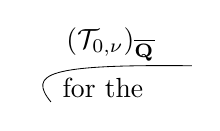
\begin{tikzpicture}[baseline=(words.base)]
\node[anchor=base west,inner sep=0] (words) at (0,0) {for the};
\node[anchor=base west,inner sep=0] at (0.05,.62) {\inserted{$(\mathcal T_{0,\nu})_{\overline{\mathbf Q}}$}};
\draw[line width=.3pt] (-.14,-.06) .. controls (-.43,.30) and (-.20,.42) .. (1.65,.40);
\end{tikzpicture} curves of genus $0$ with $\nu$ marked points, and \deleted{of the} modular \deleted{\unsure{by}} $\nu$-punctured family over $\mathcal T_{0\nu}$\ldots.

The Topos $(\mathcal T_{0,\nu})_{\mathbf Q}$ for $\nu=0,1,2$ \uline{is} not an étendue --- for the Isom schemes \unsure{of a|of a} projective bundle $X/S$ of rank $1$, with $\unsure{2|\nu}$ marked sections (distinct on each fiber). is smooth of relative dimension $3-\nu\deleted{\unsure{\geq|=|\leq}}>0$ (if $\deleted{\unsure{\nu}}0\leq\nu\leq2$).
\deleted{\unsure{Nevertheless}} \inserted{In fact} these are the toposes
\figure{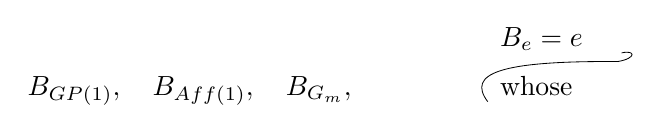
\begin{tikzpicture}[baseline=(list.base)]
\node[anchor=base west,inner sep=0] (list) at (0,0) {$B_{\operatorname{GP}(1)},\quad B_{\operatorname{Aff}(1)},\quad B_{G_m},$};
\node[anchor=base west,inner sep=0] at (6.0,0) {whose};
\node[anchor=base west,inner sep=0] at (6.0,.62) {$\inserted{B_e=e}$};
\draw[line width=.3pt] (5.85,-.08) .. controls (5.58,.28) and (6.0,.44) .. (7.5,.43) .. controls (7.74,.47) and (7.73,.58) .. (7.55,.54);
\end{tikzpicture}}
\mspage{26}
